\chapter{Arrays}
\label{ch:arrays}

\begin{goals}
\item Understand why arrays are useful
\item Learn how to use arrays in Java
\item Understand multi-dimensional arrays
\end{goals}

In Chapter \ref{chap:control}, we wrote a program which could take a numerical grade from the user, and output the corresponding letter grade. What if we wanted to include this program in a larger piece of software, which is used to make report cards for a whole class?

In principle, it's a simple idea. The steps for the previous program were as follows:
\begin{itemize}
    \item Create a variable to store the numeric grade, \ic{int grade}
    \item Use a Scanner to read in the value of \ic{grade}
    \item Use control structures to output the corresponding letter grade
\end{itemize}
We could wrap all this code in a \ic{for} loop to repeat it once for each student, but then we'll overwrite the \ic{grade} variable each time. To make report cards, we probably want to store all the grades at once, each in their own variables. So we'd have to do something like
\begin{itemize}
    \item Create a variable to store the first student's grade, \ic{int gradeOne}
    \item Create a variable to store the second student's grade, ic{int gradeTwo}
    \item Create a variable $\ldots$
\end{itemize}
Clearly this is going to get tiresome. There must be a better way.

Indeed, this is the purpose of \emph{arrays}: to declare many variables at the same time. We think of an array as a list of variables. Arrays are excellent tools for working with data in your programs, as we'll see below.

\section{Arrays in Java}

Remember, in Java, every variable has a \emph{type}. Arrays have types too, but these types are derived from other types: we could have an array of \ic{int}s, or an array of \ic{Strings}s, or an array of \ic{double}s. To tell Java we want an array, we take the type of the variables inside the array, and then put square brackets after it. So an array of \ic{int}s has type \ic{int[]}, an array of \ic{String}s has type \ic{String[]}, and an array of \ic{double}s has type \ic{double[]}.

When Java makes an array, such as an \ic{int[]}, it's really making a bunch of \ic{int}s. This means we need to tell it how long the array is, so it knows how many variables to create. One way to do this is using the \ic{new} keyword, which we've used before to create \ic{Scanner}s. Now we'll use it to create arrays. To create an array storing five \ic{int}s, we would say
\begin{code}
int[] arr = new int[5];
\end{code}
Another way to tell Java how long an array is would be to directly tell it what the values are. To do this, we place the values in a comma-separated list, inside curly braces:
\begin{code}
String[] cars = {"Volvo", "BMW", "Ford", "Mazda"};
\end{code}

\begin{example}
Write code which creates an array \ic{xs} of integers containing values 0, 2, 4, 5, 9, 13. Then write another line which creates an array \ic{ys} of seven doubles.

\noindent\emph{Answer}: To create the array of integers, we can use the curly-brace syntax:
\begin{code}
int[] xs = {0, 2, 4, 5, 9, 13};
\end{code}
\safemarginnote{This is the only time you'll see curly braces \ic{\{\}} used with arrays. For everything else, arrays use square braces, \ic{[]}.}
To create the array of doubles, we can use the \ic{new} keyword:
\begin{code}
double[] ys = new double[7];
\end{code}
\end{example}

If we tell Java how long an array is, using the \ic{new} keyword, then later on we can go in and set the values of each individual array element. To access individual array elements, we use square braces again: \ic{xs[i]} tells Java we're referring to the $i$th element of \ic{xs}. The integer $i$ is called the \emph{index}. It's important to take note of this detail: array indices start counting at 0. So, to set the first element of an array, we would use \ic{xs[0]}. To set the last element of an array of length 5, we would use \ic{xs[4]}, because the five elements are \ic{xs[0]}, \ic{xs[1]}, \ic{xs[2]}, \ic{xs[3]}, and \ic{xs[4]}. This is shown in Figure \ref{fig:array_diagram}.

\begin{figure}
    \centering
    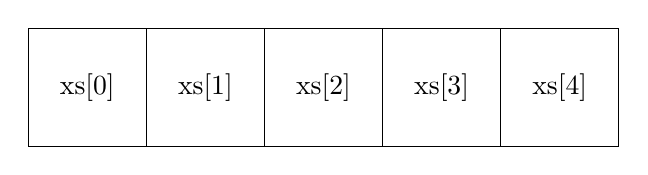
\begin{tikzpicture}[scale=1.5]
        \draw (0,0) grid (5, 1);
        \foreach \i in {0,...,4} {
            \node at ({\i+0.5},0.5) {\ic{xs[\i]}};
        };
    \end{tikzpicture}
    \caption{The elements of an array \ic{xs} of length 5.}
    \label{fig:array_diagram}
\end{figure}

\begin{example}
Write code which creates an integer array of length 4, and then sets the values to 5, 3, 8, and 7.

\noindent\emph{Answer}: The following diagram shows the code on the left, and what happens to the array on the right.
\begin{center}
    \begin{tabular}{l|c}
        \ic{int[] xs = new int[4];} & \tikz[baseline=(current bounding box.center)]{\draw (0,0) grid (4,1);} \\[2em]
        \ic{xs[0] = 5;} & \tikz[baseline=(current bounding box.center)]{\draw (0,0) grid (4,1); \node at (0.5,0.5) {5};}\\[2em]
        \ic{xs[1] = 3;} & \tikz[baseline=(current bounding box.center)]{\draw (0,0) grid (4,1); \node at (0.5,0.5) {5}; \node at (1.5, 0.5) {3};}\\[2em]
        \ic{xs[2] = 8;} & \tikz[baseline=(current bounding box.center)]{\draw (0,0) grid (4,1); \node at (0.5,0.5) {5}; \node at (1.5, 0.5) {3}; \node at (2.5, 0.5) {8};}\\[2em]
        \ic{xs[3] = 7;} & \tikz[baseline=(current bounding box.center)]{\draw (0,0) grid (4,1); \node at (0.5,0.5) {5}; \node at (1.5, 0.5) {3}; \node at (2.5, 0.5) {8}; \node at (3.5, 0.5) {7};}
    \end{tabular}
\end{center}
\end{example}

In addition to setting the values of an array, we can use the same syntax to access those values. For example, what if we want to print out the first value of an array? We could use the following code:
\begin{code}
String[] cars = {"Volvo", "BMW", "Ford", "Mazda"};
System.out.println(cars[0]);
\end{code}
This will output \ic{Volvo}.

Just like regular variables, arrays can be set and then modified. For example, consider the following code:
\begin{code}
String[] cars = {"Volvo", "BMW", "Ford", "Mazda"};
cars[0] = "Opel";
System.out.println(cars[0]);
\end{code}
At first, \ic{cars[0]} is set to \ic{"Volvo"} using the curly-brace initialization. Afterwards, we change \ic{cars[0]} to \ic{"Opel"}. Thus, when we print \ic{cars[0]}, we will see \ic{Opel}.

\begin{exercise}
Fill in the array diagram on the right on each line to track what happens to the array \ic{arr}. Write down what is printed after each print statement.
\begin{center}
    \begin{tabular}{l|c}
        \ic{int[] arr = {3, 1, 4, 1, 5};} & \tikz[baseline=(current bounding box.center),scale=0.8]{\draw (0,0) grid (5,1);} \\[2em]
        \ic{System.out.println(arr[2]);} & \underline{\hspace{1.5in}} \\[2em]
        \ic{arr[3] = 7;} & \tikz[baseline=(current bounding box.center),scale=0.8]{\draw (0,0) grid (5,1);} \\[2em]
        \ic{arr[1] = arr[2] + arr[4];} & \tikz[baseline=(current bounding box.center),scale=0.8]{\draw (0,0) grid (5,1);} \\[2em]
        \ic{System.out.println(arr[1]);} & \underline{\hspace{1.5in}} \\[2em]
        \ic{arr[0] = arr[3] - arr[0];} & \tikz[baseline=(current bounding box.center),scale=0.8]{\draw (0,0) grid (5,1);} \\[2em]
    \end{tabular}
\end{center}

\end{exercise}

% Arrays are used to store multiple values in a single variable, instead of declaring separate variables for each value.

% To declare an array, define the variable type with square brackets:

% \begin{code}
% String[] cars;
% \end{code}

% We have now declared a variable that holds an array of strings. To insert values to it, we can use an array literal - place the values in a comma-separated list, inside curly braces:

% \begin{code}
% String[] cars = {"Volvo", "BMW", "Ford", "Mazda"};
% \end{code}

% To create an array of integers, you could write:

% \begin{code}
% int[] myNum = {10, 20, 30, 40};
% \end{code}

% You access an array element by referring to the index number. This statement accesses the value of the first element in cars:
% \begin{code}
% String[] cars = {"Volvo", "BMW", "Ford", "Mazda"};
% System.out.println(cars[0]);
% // Outputs Volvo
% \end{code}

% Note that in Java (and many other programming languages) the first array element is 0 rather than 1! This is a bit unintuitive, and the source of many coding bugs. 

% \begin{figure}
% 	\centering
% 	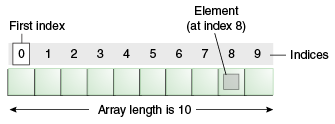
\includegraphics[width=0.5\textwidth]{images/array-diagram.png}
% 	\caption{Diagram of an array (Credit: https://www.geeksforgeeks.org/arrays-in-java/)}
% \end{figure}

% To change the value of a specific element, refer to the index number:

% \begin{code}
% String[] cars = {"Volvo", "BMW", "Ford", "Mazda"};
% cars[0] = "Opel";
% System.out.println(cars[0]);
% // Now outputs Opel instead of Volvo
% \end{code}

% To find out how many elements an array has, use the length property:

% \begin{code}
% String[] cars = {"Volvo", "BMW", "Ford", "Mazda"};
% System.out.println(cars.length);
% // Outputs 4
% \end{code}

\section{Arrays and Loops}

Let's return to the example we started the chapter with, writing report card software. Now that we know about arrays, we can avoid declaring a large number of variables by hand. Instead, we can create a single array variable, \ic{grades}, which stores each grade as an element. But how will we fill in the elements of this array? We probably want input from the user, so we can use a \ic{Scanner}. But then, we would need to write a line of code for every grade we input:
\begin{code}
Scanner input = new Scanner(System.in);
int[] grades = new int[100];
grades[0] = input.nextInt();
grades[1] = input.nextInt();
// Many more lines...
grades[99] = input.nextInt();
\end{code}
So many lines! This is exactly the kind of problem we were able to avoid with loops.

In order to use loops with arrays, we will need to access array elements using a variable. The key point to recognize is that, rather than saying \ic{grades[0]} directly, you could also define an \ic{int} which stores 0, and then use this \ic{int} as the index:
\begin{code}
int[] xs = {6, 2, 3, 4, 1};
int i = 0;
System.out.println(xs[i]);
\end{code}
There's no reason to do this if you only want the first element; but if you want to loop through every element of the array, this is very useful. For example, we could use a \ic{for} loop to set the values of the \ic{grades} array:
\begin{code}
Scanner input = new Scanner(System.in);
int[] grades = new int[100];
for(int i = 0; i < 100; i++) {
    grades[i] = input.nextInt();
}
\end{code}
This does the exact same thing as the code above, but without needing 100 lines.

Let's look carefully at how the \ic{for} loop is set up. We want to access the variables \ic{grades[0]}, \ic{grades[1]}, all the way through \ic{grades[99]} (but not \ic{grades[100]} -- this would be the 101\textsuperscript{st} element, which doesn't exist!). This means that our index variable \ic{i} should start at 0, and increase by 1 at each step, but always stay less than 100. This is how we set up the \ic{for} loop. In general, to loop through an array, you can use a loop like\marginnote{Your index variable can be called anything you'd like, but it's very common to use \ic{i}.}
\begin{code}
for(int i = 0; i < (*put length of array here*); i++)
\end{code}

\begin{example}Where is the bug in this code?
\begin{code}
int[] arr = new int[100]; 
for (int i = 0; i <= 100; ++i) {
    System.out.println(arr[i]);
}
\end{code}
\noindent \emph{Answer}:
In the last iteration of the loop, when \ic{i = 100}, the program attempts to access the value \ic{arr[100]}, but the last element in the array is \ic{arr[99]}.\safemarginnote{This kind of bug is so common, it has its own name: it's called an ``off-by-one error.'' In general, an off-by-one error is one in which a loop iterates one time too many or too few.}

If you have this bug in your code, Java will not catch it when you compile the code. Your code will run, but then Java will halt and throw an \ic{ArrayOutOfBoundsException}. When you see this message when your code runs, you know you've tried to access an element of an array which doesn't exist.
\end{example}

Instead of typing in the length of the array directly, you can use \ic{arr.length} to get the length of an array called \ic{arr}. For example, the following \ic{for} loop will print out all the \ic{String}s in the \ic{cars} array.
\begin{code}
String[] cars = {"Volvo", "BMW", "Ford", "Mazda"};
for (int i = 0; i < cars.length; i++) {
  System.out.println(cars[i]);
}
\end{code}
If you were to add another element to the \ic{cars} array, you wouldn't have to change the \ic{for} loop to reflect this: since it uses \ic{cars.length} directly, it will always iterate over the entire array, no matter how long it is.

\begin{example}
Use a \ic{for} loop to create an array of length 1000 which stores the numbers 0 through 999, in that order.

\noindent\emph{Answer}: We can set each element of the array in a \ic{for} loop, like this:\safemarginnote{Note that we're using the variable \ic{n} to set the length of the array. This is useful when we need to create an array, but we don't know from the start how long it should be -- for example, if the user tells us at runtime how many values they'd like to store.}
\begin{code}
int n = 1000;
int[] numbersArray = new int[n];
for (int i=0; i < numbersArray.length; i++) {
  numbersArray[i]=i;
}
\end{code}
\end{example}

\begin{example}
What are the values of the integer array \ic{arr} by the end of this code snippet? 
\begin{code}
    int n = 6;
    
    int[] arr = new int[n];
    for (int i = 0; i < n; i++) {
      arr[i] = i;
    }

    for (int i = 0; i < arr.length/2; i++) {
      int tmp = arr[i];
      arr[i] = arr[arr.length-1-i];
      arr[arr.length-i-1] = tmp;
    }
\end{code}

\noindent \emph{Answer}:
Let's work this out step by step. The first \ic{for} loop is just like the previous example: it sets up \ic{arr} to store the values 0 through 5, so the array starts off as
\begin{center}
    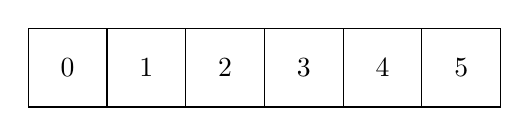
\begin{tikzpicture}
        \draw (0,0) grid (6, 1);
        \foreach \i in {0,...,5} {
            \node at ({\i+0.5}, 0.5) {\i};
        };
    \end{tikzpicture}
\end{center}
Now let's work through the first iteration of the next \ic{for} loop. The loop variable \ic{i} starts as 0, and so \ic{tmp} is set to the value of \ic{arr[0]}, which is 0. Then the next line sets \ic{arr[0]} to \ic{arr[6-1-0]}, which is \ic{arr[5]}, or 5. So now the array is
\begin{center}
    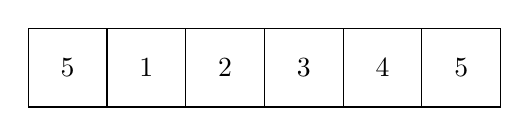
\begin{tikzpicture}
        \draw (0,0) grid (6, 1);
        \node at (0.5, 0.5) {5};
        \foreach \i in {1,...,5} {
            \node at ({\i+0.5}, 0.5) {\i};
        };
    \end{tikzpicture}
\end{center}
On the next line, we set the value of \ic{arr[5]} to \ic{tmp}, which was 0. So after the first iteration, the array is
\begin{center}
    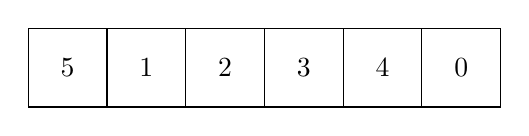
\begin{tikzpicture}
        \draw (0,0) grid (6, 1);
        \node at (0.5, 0.5) {5};
        \node at (5.5, 0.5) {0};
        \foreach \i in {1,...,4} {
            \node at ({\i+0.5}, 0.5) {\i};
        };
    \end{tikzpicture}
\end{center}
Let's take a step back: what happened to the array? We swapped the first element and the last element. Looking in detail at the code, we see that each iteration of the loop swaps the \ic{i}th element with the \ic{(arr.length-i-1)}th element. So, on the next iteration, we swap \ic{arr[1]} and \ic{arr[4]}. On the iteration afterwards, we swap \ic{arr[2]} and \ic{arr[3]}. And that's it -- the \ic{for} loop stops here, because the constraint says \ic{i < arr.length/2}, and \ic{arr.length/2} is 3. So, after the code is finished, the array is
\begin{center}
    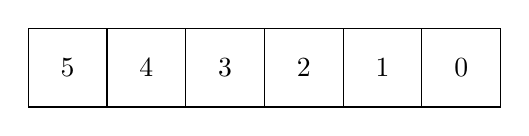
\begin{tikzpicture}
        \draw (0,0) grid (6, 1);
        \foreach \i in {0,...,5} {
            \node at ({5.5-\i}, 0.5) {\i};
        };
    \end{tikzpicture}
\end{center}
\end{example}

% There is also a "for-each" loop, which is used exclusively to loop through elements in arrays:

% \begin{code}
% for (type variable : arrayname) {
%   ...
% }
% \end{code}

% The following example outputs all elements in the cars array, using a "for-each" loop:

% \begin{code}
% String[] cars = {"Volvo", "BMW", "Ford", "Mazda"};
% for (String i : cars) {
%   System.out.println(i);
% }
% \end{code}

% The example above can be read like this: for each String element (called i - as in index) in cars, print out the value of i.

% If you compare the for loop and for-each loop, you will see that the for-each method is easier to write, it does not require a counter (using the length property), and it is more readable.

\section{Multidimensional Arrays}

Let's think carefully about what we've learned about array types. Whenever we have a variable type in Java, like \ic{int}, we can form an array type from it, like \ic{int[]}. More generally, if we have some type \ic{T}, we can always form an array type \ic{T[]}, which is an array of elements of type \ic{T}.

We can apply this same logic back to array types themselves. For example, since \ic{int[]} is a type, we can form an array of \ic{int[]}s, using the \ic{int[][]} type.

What does this kind of array look like? Let's start by initializing one. We can use curly braces to set the values of the array, but then each element is also an array, so we use nested curly braces, like this:
\begin{code}
int[][] myNumbers = { {1, 2, 3, 4}, {5, 6, 7} };
\end{code}
Now \ic{myNumbers.length} is 2, since we gave the array 2 elements. But since \ic{myNumbers[0]} is also an array, it has a length also: \ic{myNumbers[0].length} is 4. Likewise, \ic{myNumbers[1].length} is 3.

If we draw this array the way we've done before, we might get something like this:
\begin{center}
    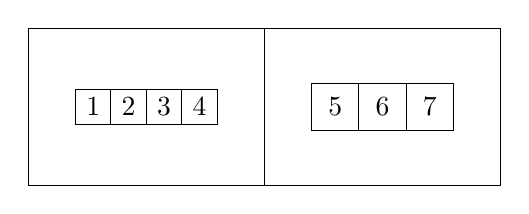
\begin{tikzpicture}
        \draw[xscale=3,yscale=2] (0,0) grid (2, 1);
        \draw[shift={(0.6,0.775)},scale=0.45] (0,0) grid (4,1);
        \draw[shift={(3.6,0.7)},scale=0.6] (0,0) grid (3,1);
        \foreach \i in {1,...,4}
            \node at ({0.825+0.45*(\i-1)},1) {\i};
        \foreach \i in {5,...,7}
            \node at ({3.9+0.6*(\i-5)},1) {\i};
    \end{tikzpicture}
\end{center}

The reason we call these ``multidimensional arrays'' is that it is often easier to draw them in another way. Typically, the entries in such an array all have the same length. That is, if our multidimensional array is \ic{xs}, then \ic{xs[0].length} is the same as \ic{xs[1].length}, \ic{xs[2].length}, and so on. This means that if we draw each element of \ic{xs} as a row of boxes like before, and stack all these rows, we get a grid. For instance, if \ic{xs.length} is 4 and \ic{xs[0].length} is 5, then we can represent the multidimensional array like this:
\begin{center}
    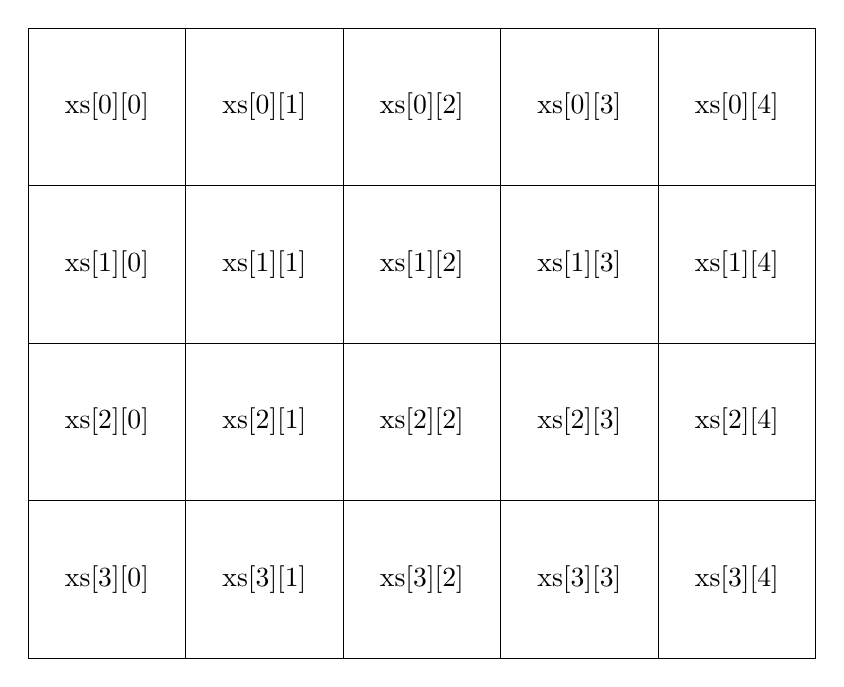
\begin{tikzpicture}[scale=2]
        \draw (0,0) grid (5,4);
        \foreach \i in {0,...,3} {
            \foreach \j in {0,...,4}  {
                \node at ({\j+.5},{3.5-\i}) {\ic{xs[\i][\j]}};
            };
        };
    \end{tikzpicture}
\end{center}
We think of the first index as the row and the second index as the column, so \ic{xs[r][c]} is the element in the \ic{r}th row and the \ic{c}th column. To initialize a multidimensional array with a grid shape, we can tell Java how many rows and how many columns there are. For instance, to initialize the array \ic{xs} drawn above, we would use
\begin{code}
int[][] xs = new int[4][5];
\end{code}

Just as with single-dimensional arrays, we can use \ic{for} loops to work with multidimensional arrays. Typically the right tool for a multidimensional array is a nested \ic{for} loop. We use one \ic{for} loop for the row index, and another \ic{for} loop for the column index. To loop over the \ic{xs} array above, we could use
\begin{code}
for(int i = 0; i < 4; i++) {
    for(int j = 0; j < 5; j++) {
        // do something to xs[i][j]
    }
}
\end{code}
Instead of explicitly specifying the bounds 4 and 5, we could also use \ic{xs.length} and \ic{xs[0].length}, respectively.

\begin{example}
What does the following code snippet do?
\begin{code}
int[][] xs = new int[8][8];
for(int i = 0; i < 8; i++) {
    for(int j = 0; j < 8; j++) {
        if((i+j) % 2 == 0) {
            xs[i][j] = 0;
        }
        else {
            xs[i][j] = 1;
        }
    }
}
\end{code}

\noindent \emph{Answer}: The \ic{for} loops will run through all pairs of indices \ic{i} and \ic{j} in the array \ic{xs}. At each position in the array, we use an \ic{if} statement to check if \ic{i+j} is divisible by 2. Using the grid picture above, try marking all the entries where the sum of the indices is divisible by 2. You should get a checkerboard pattern. If you carry this out for the full $8\times 8$ grid \ic{xs}, you should find the following pattern of ones and zeroes:
\begin{center}
    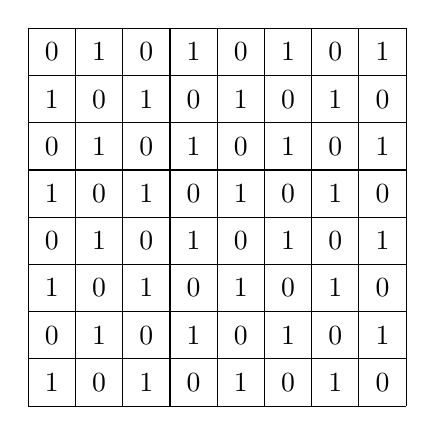
\begin{tikzpicture}[scale=.6]
        \draw (0,0) grid (8,8);
        \foreach \i in {0,...,7} {
            \foreach \j in {0,...,7} {
                \node at ({7.5-\i},{0.5+\j}) {\pgfmathparse{int(mod(\i+\j,2))}\pgfmathresult};
            };
        };
    \end{tikzpicture}
\end{center}
\end{example}

\exercisesection

\begin{exercise}
Point out all four errors in the following code snippet, and rewrite the code so that it will compile.

\begin{code}
int xs = {3, 5, 7, 8};
xs[1] = xs[2] + xs[4];
for(int i = 0; i <= 4; i++) {
    xs[i] = xs[i] + 1;
}
for(int i = 3; i >= 0; i--) {
    System.out.println(xs{i});
}
\end{code}
\end{exercise}

\begin{exercise}
What are the entries of the array \ic{cars} after the following code runs?
\begin{code}
String[] cars = {"Mazda", "Chevy", "Ford", "Toyota", "Honda"};
for(int i = 0; i < 4; i++) {
    cars[i] = cars[i+1];
}
\end{code}
\end{exercise}

\begin{exercise}
Draw the array \ic{xs} as a grid after the following code runs.
\begin{code}
int[][] xs = new int[4][6];
for(int i = 0; i < 4; i++) {
    for(int j = 0; j < 6; j++) {
        xs[i][j] = i*j - i - j;
    }
}
\end{code}
\end{exercise}

% Consider this snippet of code:

% \begin{code}
% if      (day ==  0) System.out.println("Monday");
% else if (day ==  1) System.out.println("Tuesday");
% else if (day ==  2) System.out.println("Wednesday");
% else if (day ==  3) System.out.println("Thursday");
% else if (day ==  4) System.out.println("Friday");
% else if (day ==  5) System.out.println("Saturday");
% else if (day ==  6) System.out.println("Sunday");
% \end{code}

% \noindent What does this code do? It prints the day of the week after conditioning on the value of an integer \ic{day}. But this code is repetitive. It would be useful if we had some way of creating a list of days of the week, and then just specifying which of those days we wanted to print. Something like this:

% \begin{code}
% System.out.println(DAYS\_OF\_WEEK[day]);
% \end{code}

% To achieve this in Java, we need arrays.

% \begin{definition}
% An \emph{array} is a fixed-length list of values that are of the same type. We can access data in an array by \emph{indexing}, which means referring to specific values in the array by number. If an array has \ic{n} values, then we think of it as being numbered from \ic{0} to \ic{n-1}.
% \end{definition}

% \begin{figure}
% 	\centering
% 	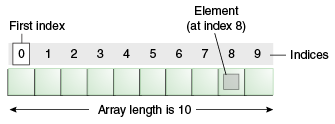
\includegraphics[width=0.5\textwidth]{images/array-diagram.png}
% 	\caption{Diagram of an array (Credit: https://www.geeksforgeeks.org/arrays-in-java/)}
% \end{figure}

% To \emph{loop} or \emph{iterate} over an array means that our program accesses every value in the array, typically in order. For example, if we looped over the array in the diagram, that would mean that we looked at the value at the 0th index, then the value at the 1st index, then the value at the 2nd index, and so on.

% Arrays are \emph{fixed-length}, meaning that after we have created an array, we cannot change its length. We will see next semester that \ic{ArrayLists} are an array-like data structure that allows for changing lengths.

% Finally, all the values in an array must be of the same type. For example, an array can hold all floating point numbers or all characters or all strings. But an array cannot hold values of different types.

% \section{Creating arrays}

% The syntax for creating an array in Java has three parts:

% \begin{enumerate}
% \item Array type
% \item Array name
% \item Either: array size or specific values
% \end{enumerate}

% For example, this code creates an array of size \ic{n = 10} and fills it with all \ic{0.0}s

% \begin{code}
% double[] arr;                    // Declare array
% arr = new double[n];             // Initialize the array
% for (int i = 0; i < n; i++) {    // Iterate over array
%     arr[i] = 0.0;                // Initialize elements to 0.0
% }
% \end{code}

% The key steps are: we first declare and initialize the array. We then loop over the array to initialize specific values. We can also initialize the array at compile time, for example

% \begin{code}
% String[] DAYS_OF_WEEK = {
% //  Indices:
% //  0      1      2      3      4      5      6
%     "Mon", "Tue", "Wed", "Thu", "Fri", "Sat", "Sun"
% };
% \end{code}

% Notice the difference in syntax. When creating an empty array, we must specify a size. When initialize an array at compile time with specific values, the size is implicit in the number of values provided.

% Finally, in Java, it is acceptable to move the brackets to directly after the type declaration to directly after the name declaration. For example, these two declarations are equivalent:

% \begin{code}
% int arr[];
% int[] arr;
% \end{code}

% \section{Indexing}

% Consider the array \ic{DAYS\_OF\_WEEK} from the previous section. We can \emph{index} the array using the following syntax:

% \begin{code}
% System.out.println(DAYS_OF_WEEK[3]);  // Prints "Thu"
% \end{code}

% In Java, array's are said to use \emph{zero-based indexing} because the first element in the array is accessed with the number \ic{0} rather than \ic{1}.

% \begin{example}
% What does \ic{System.out.println(DAYS\_OF\_WEEK[1]);} print?
% \end{example}

% \begin{example}
% What does this code do? What number does it print?

% \begin{code}
% double sum = 0.0;
% double[] arr = { 1, 2, 2, 3, 4, 7, 9 }
% for (int i = 0; i < arr.length; i++) {
%     sum += arr[i];
% }
% System.out.println(sum / arr.length);
% \end{code}
% \end{example}

% \section{Array length}

% As mentioned previously, arrays are \emph{fixed-length}. After you have created an array, it's length is unchangeable. You can access the length of an array \ic{arr[]} with the code \ic{arr.length}.

% \begin{example}
% What does \ic{System.out.println(DAYS\_OF\_WEEK.length);} print?
% \end{example}

% \begin{example}
% Write a \ic{for} loop to print the days of the week in order (Monday through Sunday) using an array rather than seven \ic{System.out.println} function calls.
% \end{example}

% \section{Default initialization}

% In Java, the default initial values for numeric primitive types is \ic{0} and \ic{false} for the \ic{boolean} type.

% \begin{example}
% Consider this code from earlier:

% \begin{code}
% double[] arr;
% arr = new double[n];
% for (int i = 0; i < n; i++) {
%     arr[i] = 0.0;
% }
% \end{code}

% Rewrite this code to be a single line.
% \end{example}

% \section{Bounds checking}

% Consider this snippet of code.

% \begin{example}Where is the bug?
% \begin{code}
% int[] arr = new int[100]; 
% for (int i = 0; i <= 100; ++i) {
%     System.out.println(arr[i]);
% }
% \end{code}
% \end{example}

% The issue is that the program attempts to access the value \ic{arr[100]}, while the last element in the array is \ic{arr[99]}.

% This kind of bug is called an ``off-by-one error'' and is so common it has a name. In general, an off-by-one-error is one in which a loop iterates one time too many or too few.

% \begin{example}
% Where is the off-by-one-error?

% \begin{code}
% int[] arr = new int[100];
% for (int i = 0; i < array.length; i++) {
%     arr[i] = i;
% }
% for (int i = 100; i > 0; --i) {
%     System.out.println(arr[i]);
% }
% \end{code}
% \end{example}

% \begin{example}
% Fill in the missing code in this \ic{for} loop to print the numbers in reverse order, i.e. \ic{5, 4, 3, 2, 1}:

% \begin{code}
% int[] arr = { 1, 2, 3, 4, 5 };
% for (???) {
%     System.out.println(arr[i]);
% }
% \end{code}
% \end{example}

% \section{Empty arrays}

% This code prints five values, one per line, but we never specified which values. What do you think it prints?

% \begin{code}
% int[] arr = new int[5];
% for (int i = 0; i < arr.length; i++) {
%     System.out.println(arr[i]);
% }
% \end{code}

% In Java, an unitialized or empty array is given a default value:

% \begin{itemize}
% \item For \ic{int}, \ic{short}, \ic{byte}, or \ic{long}, the default value is \ic{0}.
% \item For \ic{float} or \ic{double}, the default value is \ic{0.0}
% \item For \ic{boolean} values, the default value is \ic{false}.
% \item For \ic{char}, the default value is the null character \ic{'\u0000'}.
% \end{itemize}

% Note that an array can be partially initialized.

% \begin{example}
% What does this code print?

% \begin{code}
% char[] alphabet = new char[26];
% alphabet[0] = 'a';
% alphabet[1] = 'b';
% for (int i = 0; i < alphabet.length; i++) {
%     System.out.println(alphabet[i]);
% }
% \end{code}
% \end{example}

% \section{Enhanced for loop}

% So far, we have seen how to iterate over arrays by indexing each element with a number:

% \begin{code}
% char[] vowels = {'a', 'e', 'i', 'o', 'u'};
% for (int i = 0; i < vowels.length; ++ i) {
%     System.out.println(vowels[i]);
% }
% \end{code}

% We can perform the same iteration without using indices using an ``enhanced \ic{for} loop'' or \ic{for-each} loops:

% \begin{code}
% char[] vowels = {'a', 'e', 'i', 'o', 'u'};
% for (char item: vowels) {
%     System.out.println(item);
% }
% \end{code}

% \section{Exchanging and shuffling}

% Two common tasks when manipulating arrays are \emph{exchanging two values} and \emph{shuffling} values. (\emph{Sorting} is more complicated and will be address later.)

% To exchange to values, consider the following code:

% \begin{code}
% double[] arr = { 1.0, 2.0, 3.0, 4.0, 5.0, 6.0 };
% int i = 1;
% int j = 4;
% double tmp = arr[i]; 
% arr[i] = arr[j]; 
% arr[j] = tmp;
% \end{code}

% \begin{example}
% What are the six values in the array, in order?
% \end{example}

% To shuffle the array, consider the following code:

% \begin{code}
% int n = arr.length; 
% for (int i = 0; i < n; i++) { 
%     int r = i + (int) (Math.random() * (n-i)); 
%     String tmp = arr[r];
%     arr[r] = arr[i];
%     arr[i] = tmp;
% }
% \end{code}

% \begin{example}
% What does this code do?

% \begin{code}
% for (int i = 0; i < n/2; i++) {
%     double tmp = arr[i];
%     arr[i] = arr[n-1-i];
%     arr[n-i-1] = tmp;
% }
% \end{code}
% \end{example}

% \exercisesection

% \begin{exercise}
% Write a program that reverses the order of values in an array.
% \end{exercise}

% \begin{exercise}
% What is wrong with this code snippet?

% \begin{code}
% int[] arr;
% for (int i = 0; i < 10; i++) {
%     arr[i] = i;
% }
% \end{code}
% \end{exercise}

% \begin{exercise}
% Rewrite this snippet using an enhanced \ic{for-each} loop (for now, it is okay to re-define the array):

% \begin{code}
% char[] vowels = {'a', 'e', 'i', 'o', 'u'};
% for (int i = array.length; i >= 0; i--) {
%     char letter = vowels[i];
%     System.out.println(letter);
% }
% \end{code}
% \end{exercise}

% \begin{exercise}
% Write a program that uses \ic{for} loops to print the following pattern:

% \begin{code}
% 1********

% 12*******

% 123******

% 1234*****

% 12345****

% 123456***

% 1234567**

% 12345678*

% 123456789
% \end{code}
% \end{exercise}

% \begin{exercise}
% Write a program \ic{HowMany.java} that takes an arbitrary number of command line arguments and prints how many there are.
% \end{exercise}

% \referencessection

% Computer Science: An Interdisciplinary Approach, Robert Sedgewick and Kevin Wayne.
